\section{CorsNet: 3D Point Cloud Registration by Deep Neural
Network}\label{header-n534}

\emph{IEEE ROBOTICS AND AUTOMATION LETTERS, VOL. 5, NO. 3, JULY 2020}
{[}12{]}

\subsection{Introduction}\label{header-n536}

In computer vision, pattern recognition, and robotics, \emph{point set
registration}, also known as \emph{point cloud registration}, is the
process of finding a spatial transformation (\emph{e.g.,} scaling,
rotation and translation) that aligns two point clouds. The 3D point
cloud is a recently popular data format. The most popular and classic
method for point cloud registration is the iterative closest point (ICP)
algorithm {[}13{]}. ICP calculates the rigid motion based on a fixed
correspondence between one point cloud and another, updating the
correspondence to minimize the point-to-point distances. Although ICP
can achieve highly accurate registration, the registration often fails
by falling into the local minimum. In other words, the registration
accuracy of ICP depends strongly on its initial perturbation. Despite
this, the inherent lack of structure has caused difficulties when
adopting point clouds as direct input in deep learning architecture.
PointNet {[}14{]}, overcomes these difficulties, providing a mechanism
to extract the feature related to the point clouds. PointNet is a
general representation of an unstructured point cloud that allows object
detection, segmentation, and so on. PointNetLK {[}15{]} is the latest
deep learning-based registration techniques using PointNet {[}2{]}.
PointNetLK directly optimizes the distance of aggregated features using
the gradient method. This approach overcomes computational speed and
local minimum problems. In this paper, ``DirectNet" is proposed as a
baseline method as it is a simplistic approach. However, the authors
think that PointNetLK and DirectNet do not consider local features,
falling to fully utilize the point cloud information. In this work,
CorrespondenceNet (CorsNet) is proposed. It is a novel point cloud
registration method based on deep learning is proposed. This method
feeds global features from PointNet to per-point local features to make
effective use of point cloud information. The end-to-end network
architecture consists of the main three parts: (1) extracting global
features of point clouds with PointNet, (2) concatenating global
features with local features of the source point cloud and outputting
the correspondences of each point via fully connected layers and (3)
estimating a rigid transform with singular value decomposition (SVD).
The SVD part is also included in the end-to-end network architecture.
The singular value decomposition is a factorization of a matrix
$m \times n$. Given the matrix here $\mathbf {M}_{m\times n}$,
$\mathbf{M} = \mathbf{U}\mathbf{\Sigma}\mathbf{V}$. If $\mathbf {M}$ is used
in a geometrical operation, the same result can be obtained applying
these three matrices in succession. In particular,
$\mathbf {U}_{m\times n}$ is an orthogonal matrix that applies a
rotation, $mathbf{\Sigma}_{n\times n}$ is a diagonal matrix that scales only
the axes and $\mathbf {V}_{n\times q}$ is another orthogonal matrix
that applies another rotation.
\newpage
\begin{figure}[h!]
\centering
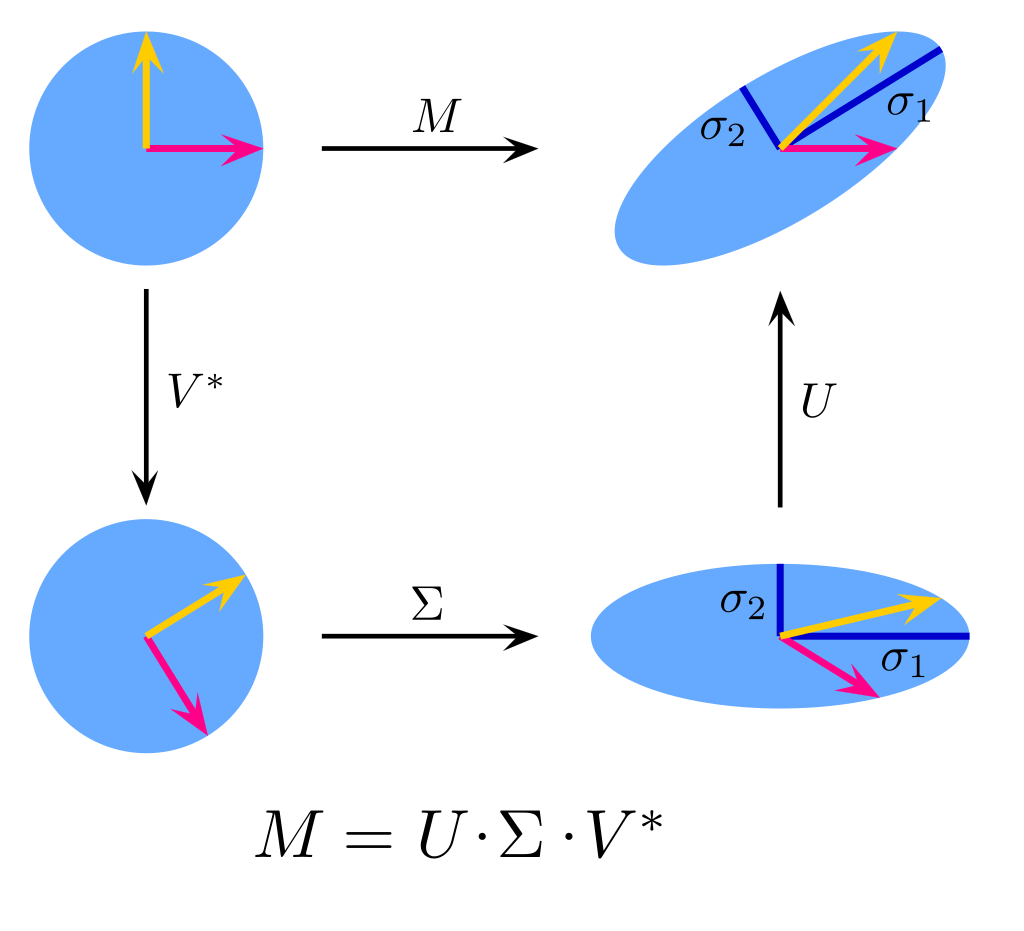
\includegraphics[width=0.7\linewidth]{images/singolarvaluedec.png}
\caption{Singular value decomposition}
\end{figure}

\subsection{Proposed method (CorsNet)}\label{header-n539}

A point cloud is represented as a set of 3D points
$\{P : P_i|i = 1, . . ., n\} \subset \R_3$ whose each point $P_i$ is
a vector of its $(x, y, z)$ coordinate. The following figure shows the
CorstNet architecture.

\begin{figure}[h!]
\centering
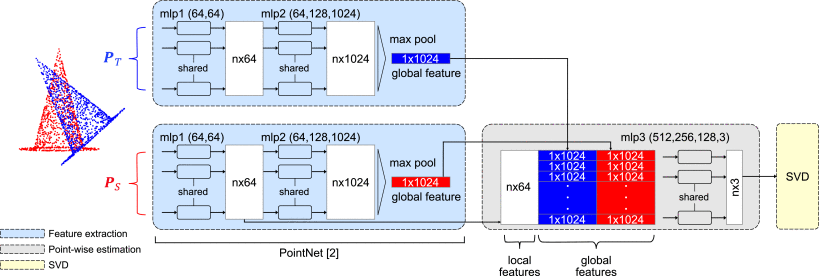
\includegraphics[width=0.8\linewidth]{images/corsnetarch.png}
\caption{CorsNet architecture}
\end{figure}

The red $\boldsymbol{P}_S$ and blue $\boldsymbol{P}_T$ point clouds
represent the \emph{source} and \emph{template} point clouds,
respectively. We find the rigid transform $\boldsymbol{G} \in SE$,
which includes the alignment between $\boldsymbol{P}_S$ and
$\boldsymbol{P}_T$. The model mainly consists of three components:

\begin{itemize}
\item
  \textbf{Global feature extraction:} this first module extract the
  point cloud's features. These features must include three factors:
  invariance in order, acquisition of local feature, and invariance in
  rotation. PointNet is used to absolve this goal. It satisfying these
  three requirements and it has achieved high accuracy and low
  computational complexity in various benchmarks. The PointNet output is
  a $1 \times 1024$ vector obtained by a max-pooling of two MLP (multi-layer
  perceptron). The features are extracted both for the source and
  template point clouds.
\item
  \textbf{Correspondence estimation:} after computing the global
  features of the source and template point cloud, this module finds the
  point local features by concatenating the global feature with each of
  the point features. The network output is t
  $\Delta\boldsymbol{P}_S$, a $n \times 3$ matrix. By adding this
  $\Delta\boldsymbol{P}_S$ to $\boldsymbol{P}_S$, the tentative
  transform destination can be calculated as follow:

  $ \hat{\boldsymbol {P}_T} = \boldsymbol {P}_S + \Delta \boldsymbol {P}_S $

  This method regresses correspondences $\Delta\boldsymbol{P}_S$ and
  estimates a rigid transform based on the estimated correspondences
  using SVD

  $ \boldsymbol {G}\cdot \boldsymbol {P}_S= \boldsymbol {P}_T$
\item
  \textbf{SVD:} the source point cloud is now aligned with the template
  point cloud and the following is the approach for calculating a rigid
  transformation using SVD as follows.

  Define the centroids of $\boldsymbol{P}_S$ and
  $\hat{\boldsymbol{P}_T}$ as:

  $\overline{\boldsymbol {P}_S} = \frac{1}{n}\sum ^{n}_{i=1}\boldsymbol {P}_S \;\;\; \text{and} \;\;\; \overline{\hat{\boldsymbol {P}_T}} = \frac{1}{n}\sum ^{n}_{i=1}\hat{\boldsymbol {P}_T}$

  and calculate the cross-covariance matrix H:

  $ \boldsymbol {H}= \sum ^{N}_{i=1}\left(\hat{\boldsymbol {P}_T}-\overline{\hat{\boldsymbol {P}_T}}\right)\left(\boldsymbol {P}_S-\overline{\boldsymbol {P}_S}\right)^{T}.$

  Then, use SVD to decompose $\boldsymbol{H}$ to
  $\boldsymbol{U},\boldsymbol{V} \in SO$

  $  [\boldsymbol {U}, \boldsymbol {S}, \boldsymbol {V}]= SVD (\boldsymbol {H}).$

  and, using this decomposition, extract the rigid transform elements,
  estimated rotation, $\boldsymbol{R}_{est}\in SO$ and translation,
  $\boldsymbol{t}_{est} \in \R^3$

  $ \boldsymbol {R}_{est} = \boldsymbol {V}\boldsymbol {U}^{T}.\\\boldsymbol {t}_{est} = - \boldsymbol {R}\cdot \overline{\hat{\boldsymbol {P}_T}} + \overline{\boldsymbol {P}_S}. $

  Now, it is possible to calculate the estimated rigid transform
  $\mathbf{G}_{est}$ and the twist parameters
  $\mathbf{\xi}_{est} \in \R^{6}$ as follow:

  $ \boldsymbol {G}_{est} = \left(\begin{array}{cc}\boldsymbol {R}_{est} & \boldsymbol {t}_{est} \\ \boldsymbol {0} & 1 \end{array} \right). \\ \boldsymbol {\xi }_{est} = \phi \left(\boldsymbol {G}_{est} \right). $
\end{itemize}

\newpage
The dataset used to test the proposed method is called ModelNet40
{[}16{]}. From this, the source point clouds ($\boldsymbol{P}_S$) are
extracted and the ground-truth estimated rigid transform
($\boldsymbol{G}_{gt}$) can be defined as:\newline\
$ \boldsymbol {P}_{T} = \boldsymbol {G}_{gt}\cdot \boldsymbol {P}_{S}.$\newline
Now, we call $\boldsymbol{Cors}$ the correspondence between two point
clouds, in particular: \newline
$\boldsymbol {Cors}_{gt} = \boldsymbol {P}_{T} - \boldsymbol {P}_{S}.  \\  \boldsymbol {Cors}_{est} = \hat{\boldsymbol {P}_{T}} - \boldsymbol {P}_{S}.$
\newline
Subsequently, we define three kinds of loss elements using previously
values:
\newline
$ \boldsymbol {loss}_{1} = ||(\boldsymbol {G}_{est})^{-1}\cdot \boldsymbol {G}_{gt} - \boldsymbol {I}_{4}||_{F}. \\ \boldsymbol {loss}_{2} = ||\boldsymbol {\xi }_{gt}-\boldsymbol {\xi }_{est}||^{2}. \\ \boldsymbol {loss}_{3} = ||\boldsymbol {Cors}_{gt} - \boldsymbol {Cors}_{est}||^{2}. $
\newline
From them, four loss functions are defined as follow:
\newline
$ \boldsymbol {Loss}_{v1} = \boldsymbol {loss}_{1}. \\ \boldsymbol {Loss}_{v2} = \boldsymbol {loss}_{2}. \\ \boldsymbol {Loss}_{v3} = \boldsymbol {loss}_{1} + \boldsymbol {loss}_{3}.\\ \boldsymbol {Loss}_{v4} = \boldsymbol {loss}_{2} + \boldsymbol {loss}_{3}.  $
\newline
The authors verified the effectiveness of each loss function in the
experiments.

\subsection{Proposed method (DirectNet)}\label{header-n572}

The authors proposed a novel method which directly regresses the pose,
including rotation $\boldsymbol{R}_{euler} ∈ \R^3 $ (Euler angle) and
translation $\boldsymbol{t} ∈ \R^3$, as shown in the following figure.

\begin{figure}[h!]
\centering
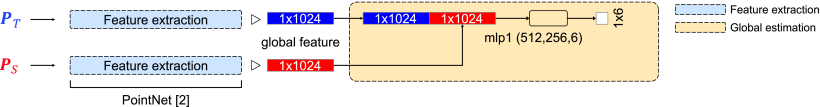
\includegraphics[width=0.95\linewidth]{images/directnet.png}
\caption{DirectNet architecture}
\end{figure}

DirectNet consists of two parts: the global feature extraction module,
which is identical to CorsNet (that is PointNet), and the global
estimation part. The $\boldsymbol{P}_S$ and $\boldsymbol{P}_T$
global features extracted with PointNet are concatenated and converted
to $1 \times 6$ vector. The output $1 \times 6$ vectors is
$[x_{euler}, y_{euler}, z_{euler}, x_{t}, y_{t}, z_{t}]^T$. The first
half of this vector is represented as
$\boldsymbol{R_{euler}} = [x_{euler}, y_{euler}, z_{euler}]^T$ . This
$\boldsymbol{R_{euler}}$ is converted into
$\boldsymbol{R_{est}} \in SO $ as follows:
\newline
$ \boldsymbol {x}_{mat} = \left(\begin{array}{ccc}1 & 0 & 0 \\ 0 & \cos x_{euler} & -\sin x_{euler} \\ 0 & \sin x_{euler} & \cos x_{euler} \end{array} \right), \\ \boldsymbol {y}_{mat} = \left(\begin{array}{ccc}\cos y_{euler} & 0 & \sin y_{euler} \\ 0 & 1 & 0 \\ -\sin y_{euler} & 0 & \cos y_{euler} \end{array} \right), \\ \boldsymbol {z}_{mat} = \left(\begin{array}{ccc}\cos z_{euler} & -\sin z_{euler} & 0 \\ \sin z_{euler} & \cos z_{euler} & 0 \\ 0 & 0 & 1 \end{array} \right), \\ \boldsymbol {R}_{est} = \boldsymbol {x}_{mat} \cdot \boldsymbol {y}_{mat} \cdot \boldsymbol {z}_{mat} $ 
\newline
The last part, instead, define the translation vector
$\boldsymbol{t_{est}}$ as
\newline
$ \boldsymbol {t}_{est} = [x_{t}, y_{t}, z_{t}]^{T}.$
\newline
Using $\boldsymbol {R}_{est}$ and $\boldsymbol {t}_{est}$ is
possible to determine $\boldsymbol {G}_{est}$ and
$\boldsymbol {\xi}_{est}$ as done for CorsNet. For DirectNet two loss
functions are formulated:
\newline
$ \boldsymbol {Loss}_{v1} = ||(\boldsymbol {G}_{est})^{-1}\cdot \boldsymbol {G}_{gt} - \boldsymbol {I}_{4}||_{F}. \\ \boldsymbol {Loss}_{v2} = ||\boldsymbol {\xi }_{gt}-\boldsymbol {\xi }_{est}||^{2}.$

\subsection{Experiments}\label{header-n581}

The proposed method CorsNet is compared with ICP and PointNetLK,
DirectNet (described in this work). The figure below shows graphical examples of pointcloud registration, each of them is executed with a different approach.

\begin{figure}[h!]
\centering
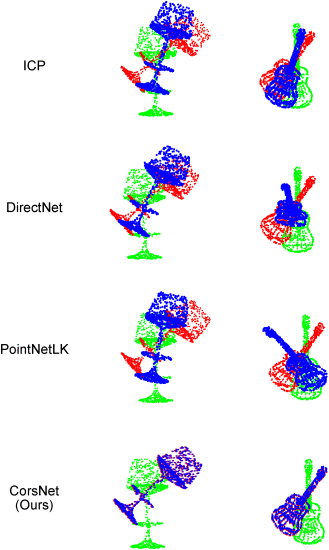
\includegraphics[width=0.4\linewidth]{images/pointcloudreg.png}
\caption{Point cloud registration. \emph{Green}: source, \emph{Blue}: template, \emph{Red}: transformed point cloud. Only the proposed method achieves accurate registration regardless of the initial perturbations.}
\end{figure}

The dataset used is ModelNet40, which includes various point clouds with
40 categories. The point clouds' coordinates are normalized to be in the
$[0, 1]^3$ interval and the points of each model's surface are
sampling to be exactly 1024. The authors measure the root mean square
error (RMSE) of rotation $\boldsymbol{R}$ and translation
$\boldsymbol{t}$ for each experimental setting. The first experiment
consists into evaluate the models using the same categories. 20
categories from the dataset were chosen and they are used for both
training and testing of all networks. CorsNet and DirectNet were trained
using all the losses reported in the sections above. The authors chose a
ground-truth transformation ($\boldsymbol{G}_{gt}$) randomly by an
interval of $[0, 45]$ degrees for rotation and $[0, 0.8]$ for
translation. The following table shows the evaluation results of all
models, using all possible loss functions.

\begin{longtable}[]{@{}lll@{}}
\toprule
\textbf{Method (loss type)} & \textbf{RMSE ($\boldsymbol{R}$)} &
\textbf{RMSE ($\boldsymbol{t}$)}\tabularnewline
\midrule
\endhead
ICP & 46.4628 & 0.26144\tabularnewline
DirectNet $\boldsymbol{Loss}_{v1}$ & 19.4791 & 0.01218\tabularnewline
DirectNet $\boldsymbol{Loss}_{v2}$ & 20.9916 & 0.01690\tabularnewline
PointNetLK & \textbf{14.9746} & 0.01690\tabularnewline
CorsNet $\boldsymbol{Loss}_{v1}$ & 18.6482 & 0.01574\tabularnewline
CorsNet $\boldsymbol{Loss}_{v2}$ & 17.9941 & 0.00725\tabularnewline
CorsNet $\boldsymbol{Loss}_{v3}$ & 18.8303 &
\textbf{0.00632}\tabularnewline
CorsNet $\boldsymbol{Loss}_{v4}$ & 16.2356 & 0.00693\tabularnewline
\bottomrule
\caption{Comparison results on same categories}
\end{longtable}

The results show that the proposed CorsNet, whose loss function is
$\boldsymbol{Loss}_{v3}$, achieved the highest accuracy in terms of
translation. The following figure shows (on its left part) the ratio
between the root mean square error with respect to perturbation both for
rotation and translation. To verify the robustness of the categories,
the authors evaluated the proposed network architecture using different
categories for training and testing. This is the second experiment. The
table below reports the performance evaluation results for the proposed
and related methods.

\begin{longtable}[]{@{}lll@{}}
\toprule
\textbf{Method (loss type)} & \textbf{RMSE ($\boldsymbol{R}$)} &
\textbf{RMSE ($\boldsymbol{t}$)}\tabularnewline
\midrule
\endhead
ICP & 45.8016 & 0.28369\tabularnewline
DirectNet $\boldsymbol{Loss}_{v1}$ & 20.8310 & 0.01983\tabularnewline
DirectNet $\boldsymbol{Loss}_{v2}$ & 22.0024 & 0.01712\tabularnewline
PointNetLK & 21.0866 & 0.03525\tabularnewline
CorsNet $\boldsymbol{Loss}_{v1}$ & 20.2198 & 0.02401\tabularnewline
CorsNet $\boldsymbol{Loss}_{v2}$ & 20.3712 & 0.02396\tabularnewline
CorsNet $\boldsymbol{Loss}_{v3}$ & 19.4610 & 0.02288\tabularnewline
CorsNet $\boldsymbol{Loss}_{v4}$ & \textbf{16.7927} &
\textbf{0.01398}\tabularnewline
\bottomrule
\caption{Comparison results on different categories}
\end{longtable}

Rotation and translation are estimated most accurately by CorsNet, whose
loss function is $\boldsymbol{Loss}_{v4}$. The following figure shows
(on its right part) the ratio between the root mean square error with
respect to perturbation both for rotation and translation.

\begin{figure}[h!]
\centering
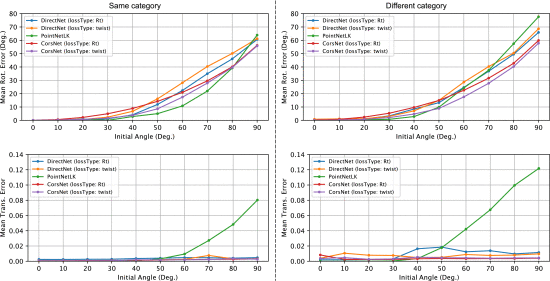
\includegraphics[width=0.95\linewidth]{images/mod.png}
\caption{Each graph shows the transition of a root mean square error with respect to the initial perturbation (rotation and translation). The left part refers to the experiments on the same category while the right part refers different categories' experiments}
\end{figure}

\subsection{Conclusions}\label{header-n662}

The superiority of the proposed method has been proven qualitatively and
quantitatively. CorsNet $\boldsymbol{Loss}_{v3}$ and CorsNet
$\boldsymbol{Loss}_{v4}$ ware appreciably more accurate thanCorsNet
$\boldsymbol{Loss}_{v1}$ and CorsNet $\boldsymbol{Loss}_{v2}$,
depending on whether the correspondence loss is included in the loss
function. The following two figure shows the registration results for
the methods tested. Only the proposed method (CorsNet) successfully
aligns the point clouds without falling into the local minimum,
especially where the input point clouds include the repeating
structures.

\begin{figure}[h!]
\centering
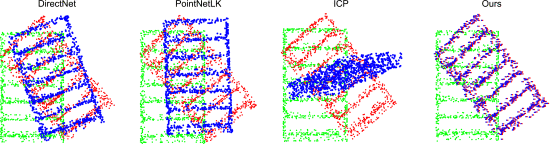
\includegraphics[width=0.95\linewidth]{images/registrationres.png}
\caption{Comparison with DirectNet, PointNetLK, and ICP (green: source, blue: template, red: transformed)}
\end{figure}

The authors suppose that this is because only the proposed method links
the local features to the global features, making the most of the local
and global point cloud information.